% A (minimal) template for problem sets and solutions using the exam document class

% Organization:
%% Define new commands, macros, etc. in macros.tex
%% Anything that you would put before \begin{document} should go in prelude.tex

%% For multiple psets, each should get its own file to \input into main with a \section{}
\documentclass[answers]{exam}
\qformat{}

\usepackage{cancel}
\usepackage{amsmath}
\usepackage{amsthm}
\usepackage{amsfonts}
\usepackage{mathtools}
\usepackage{amssymb}
\usepackage{mathrsfs}
\usepackage{graphicx}
\usepackage{enumitem}
\renewcommand{\qedsymbol}{$\blacksquare$}

\newcommand{\R}{\mathbb{R}}
\newcommand{\C}{\mathbb{C}}
\newcommand{\Z}{\mathbb{Z}}
\newcommand{\N}{\mathbb{N}}
\newcommand\tab[1][1cm]{\hspace*{#1}}
\newcommand{\K}{\mathbb{K}}
\newcommand{\zero}{\mathbb{O}}
\begin{document}

\title{Fourier Analysis and Wavelets\\Homework 3}
\author{Francisco Jose Castillo Carrasco}
\date{\today}
\maketitle

%% \union - Example: \union{j \in J}{A_j}
\newcommand{\union}[2]{\underset{#1}\bigcup #2}

%% \inter - like \union, but with \bigcap
\newcommand{\inter}[2]{\underset{#1}\bigcap #2}

%% Content goes here

\section*{Problem 5}
\begin{questions}

\question{
Using von Neumann stability analysis, show that Lax-Wendroff is
stable for $u_t + c u_x = 0$ as long as the CFL condition $r \le 1$ is
satisfied.  {\em Hint:}\/ Show $|G(k)|^2 = G^*(k) G(k) \le 1$ iff $r
\le 1$.
}
\begin{solution}

\end{solution}
\end{questions}


\section*{Problem 7}
\begin{questions}

\question{Establish the parts of \textsl{Theorem 2.6} that deal with the inverse Fourier transform. Establish the relationship between the Fourier transform and the Laplace transform given in the last part of this theorem.
}
\begin{solution}
\begin{itemize}
\item \textbf{1.} The inverse Fourier transform is a linear operator. 

\textit{Proof:}
\begin{align*}
\mathcal{F}^{-1}[\alpha f+\beta g](t)&=\frac{1}{\sqrt{2\pi}}\int_{-\infty}^{\infty}[\alpha f(\lambda)+\beta g(\lambda)]e^{i\lambda t}d\lambda\\
&=\frac{1}{\sqrt{2\pi}}\int_{-\infty}^{\infty}[\alpha f(\lambda)]e^{i\lambda t}d\lambda+\frac{1}{\sqrt{2\pi}}\int_{-\infty}^{\infty}[\beta g(\lambda)]e^{i\lambda t}d\lambda\\
&=\alpha\frac{1}{\sqrt{2\pi}}\int_{-\infty}^{\infty} f(\lambda)e^{i\lambda t}d\lambda+\beta\frac{1}{\sqrt{2\pi}}\int_{-\infty}^{\infty}g(\lambda)e^{i\lambda t}d\lambda\\
&=\alpha \mathcal{F}^{-1}[f](t)+\beta \mathcal{F}^{-1}[g](t)
\end{align*}
\item \textbf{3.} The inverse Fourier transform of a product of $f$ with $\lambda^n$ is given by
\begin{align*}
\mathcal{F}^{-1}[\lambda^nf(\lambda)](t)=(-i)^n\frac{d^n}{dt^n}\left\lbrace\mathcal{F}^{-1}[f](t)\right\rbrace
\end{align*}

\textit{Proof:}
We start with the definition of the inverse transform
\begin{align*}
\mathcal{F}^{-1}[\lambda^nf(\lambda)](t)=\frac{1}{\sqrt{2\pi}}\int_{-\infty}^{\infty}\lambda^nf(\lambda)e^{i\lambda t}d\lambda.
\end{align*}
Using
\begin{align*}
\lambda^nf(\lambda)e^{i\lambda t}=(-i)^n\frac{d^n}{dt^n}\left\lbrace f(\lambda)e^{i\lambda t}\right\rbrace,
\end{align*}
we get
\begin{align*}
\mathcal{F}^{-1}[\lambda^nf(\lambda)](t)&=\frac{1}{\sqrt{2\pi}}\int_{-\infty}^{\infty}(-i)^n\frac{d^n}{dt^n}\left\lbrace f(\lambda)e^{i\lambda t}\right\rbrace d\lambda\\
&=(-i)^n\frac{d^n}{dt^n}\left\lbrace\frac{1}{\sqrt{2\pi}}\int_{-\infty}^{\infty} f(\lambda)e^{i\lambda t} d\lambda\right\rbrace\\
&=(-i)^n\frac{d^n}{dt^n}\left\lbrace \mathcal{F}^{-1}[f](t) \right\rbrace,
\end{align*}
and complete the proof.
\item \textbf{5.} The inverse Fourier transform of the $n$th derivative of $f$ is given by
\begin{align*}
\mathcal{F}^{-1}[f^{(n)}(\lambda)](t)=(-it)^n\mathcal{F}^{-1}[f](t)
\end{align*}
\textit{Proof:}
We start with the definition of the inverse transform
\begin{align*}
\mathcal{F}^{-1}[f^{(n)}(\lambda)](t)=\frac{1}{\sqrt{2\pi}}\int_{-\infty}^{\infty}f^{(n)}(\lambda)e^{i\lambda t}d\lambda.
\end{align*}
Integrating by parts, using $u=e^{i\lambda t}$ and $dv=f^{(n)}(\lambda)d\lambda$, we get
\begin{align*}
\frac{1}{\sqrt{2\pi}}\int_{-\infty}^{\infty}f^{(n)}(\lambda)e^{i\lambda t}d\lambda=\left.\frac{1}{\sqrt{2\pi}}f^{(n-1)}(\lambda)e^{i\lambda t}\right|_{-\infty}^{\infty}-\frac{1}{\sqrt{2\pi}}\int_{-\infty}^{\infty}(it)f^{(n-1)}(\lambda)e^{i\lambda t}d\lambda.
\end{align*}
Since $f$ vanishes at $\pm\infty$ by hypothesis, there are no boundry terms. Hence,
\begin{align*}
\mathcal{F}^{-1}[f^{(n)}(\lambda)](t)&=-\frac{1}{\sqrt{2\pi}}\int_{-\infty}^{\infty}(it)f^{(n-1)}(\lambda)e^{i\lambda t}d\lambda\\
&=-(it)\frac{1}{\sqrt{2\pi}}\int_{-\infty}^{\infty}f^{(n-1)}(\lambda)e^{i\lambda t}d\lambda\\
&=-(it)\mathcal{F}^{-1}[f^{(n-1)}(\lambda)](t)
\end{align*}
where we see that there is a transfer derivatives to factors $-it$. Repeating this process $n-1$ times we obtain
\begin{align*}
\mathcal{F}^{-1}[f^{(n)}(\lambda)](t)&=(-it)^n\mathcal{F}^{-1}[f](t)
\end{align*}
\item \textbf{8.} If $f(t)=0$ for $t<0$, then
\begin{align*}
\mathcal{F}[f](\lambda)=\frac{1}{\sqrt{2\pi}}\mathcal{L}[f](i\lambda),
\end{align*}
where $\mathcal{L}[f]$ is the Laplace transform of $f$ defined by
\begin{align*}
\mathcal{L}[f](s)=\int_{0}^{\infty}f(t)e^{-ts}dt.
\end{align*}
\textit{Proof:}
We start with the definition of the Fourier transform using the assumption that the function is zero in the left half plane,
\begin{align*}
\mathcal{F}[f](\lambda)&=\frac{1}{\sqrt{2\pi}}\int_{-\infty}^{\infty}f(t)e^{-i\lambda t}dt\\
&=\frac{1}{\sqrt{2\pi}}\int_{-\infty}^{\infty}f(t)e^{-i\lambda t}dt.
\end{align*}
Using the change $s=i\lambda$ we get the desired result
\begin{align*}
\mathcal{F}[f](\lambda)&=\frac{1}{\sqrt{2\pi}}\int_{-\infty}^{\infty}f(t)e^{-i\lambda t}dt\\
&=\frac{1}{\sqrt{2\pi}}\int_{-\infty}^{\infty}f(t)e^{ts}dt\\
&=\frac{1}{\sqrt{2\pi}}\mathcal{L}[f](s)\\
&=\frac{1}{\sqrt{2\pi}}\mathcal{L}[f](i\lambda)\\
\end{align*}
\end{itemize}
\end{solution}
\end{questions}


\section*{Problem 12}
\begin{questions}

\question{
}
\begin{solution}

\end{solution}
\end{questions}

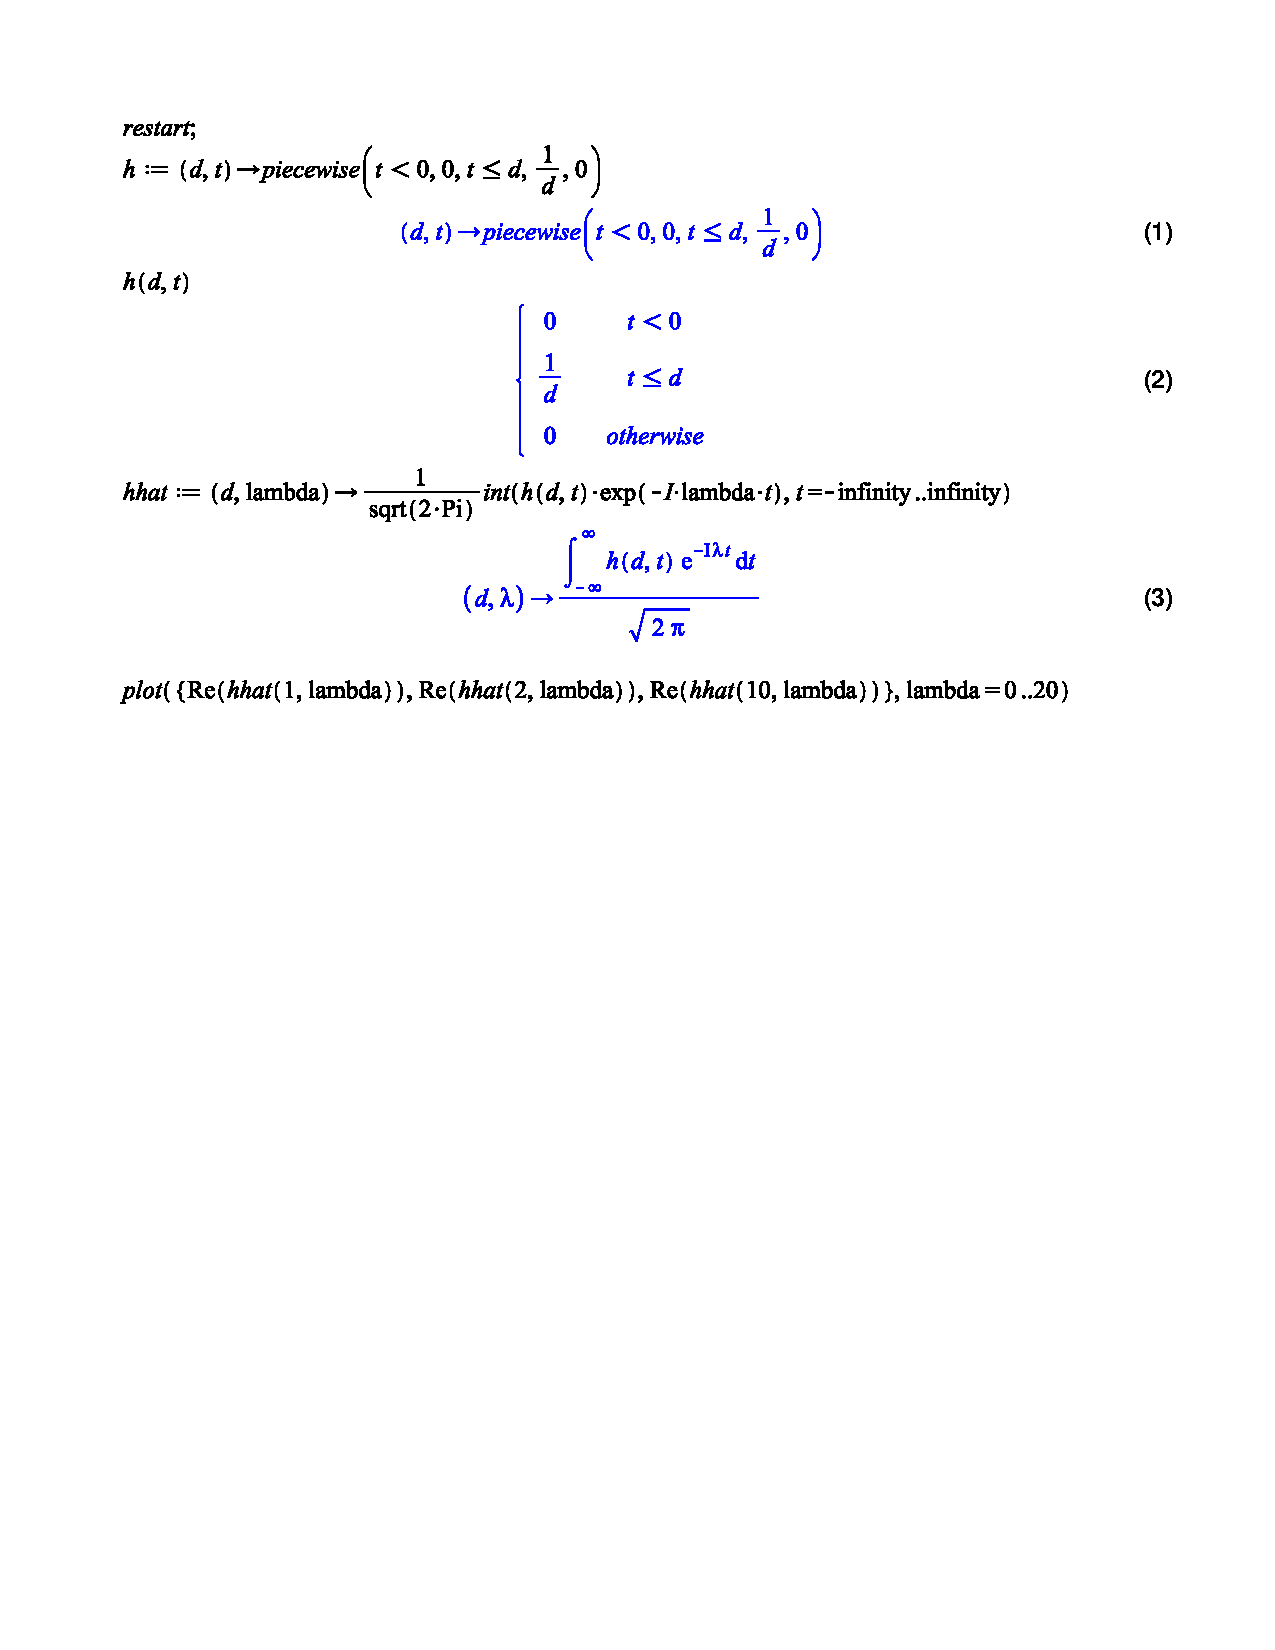
\includepdf[pages=-]{problem12}
\end{document}
